%%%%
\section{Identificação das fontes}

No artigo publicado em 2013 intitulado
\textit{Chemical composition and sources of particle pollution in affluent and
poor neighborhoods of Accra, Ghana} \citep{zhou2013} e \citep{zhou2014} 
realizou-se levantamento de 
fontes usando PMF com todas as 2898 amostras coletadas no XX sítios de 
amostragem. As fonte encotradas com seus repectivos elementos foram: 
queima de lixo sólido (Br, Pb), poeira de solo e veículo (Al, Si, Ca, Fe, Zn, 
BC, Pb), solo (Al, Si, Mg, Ti, Mn, Fe), queima de biomassa (K, Cl, S, BC) e mar 
(Na, Cl, S). Estas fontes foram encontradas para os 4 bairros (XX sítios de 
coleta) do experimento e portanto a escolha desses fatores foi realizadas de 
forma que fosse comuns as 4 regiões, portanto é um resultado genérico sobre 
Acra. Segue-se análise detalhada de um dos bairros, Nima, que além do PMF
também utiliza-se Análise de Fatores para levantamento de fontes principais. 

\citet{ARKU2008} e \citet{DIONISIO2010} foram pioneiros em conduzir  
levantamento dos níveis de poluição, composição elementar e 
distribuição espacial e temporal de poluentes em Gana.

A tabela \ref{table:cookfuel} reporta fontes de energia usadas em Gana e em
Acra usadas para preparação de alimentos e pode ajudar na identificação dos 
fatores de PMF e Análise de Fatores.
\begin{table}[H]
 \centering
  \input{../outputs/census_cookfuel.tex}
  \caption{Fontes de energia usadas para cozimento de alimentos em 
           Gana \citep{ghanacensus2013} \label{table:cookfuel}}
\end{table}

No mapa da figura \ref{fg:acrasources} foram marcadas possíveis fontes 
poluídoras locais de Acra, também para ajudar na identificação dos fatores. 

\begin{figure}[H]
  \centering
  \caption{Levantamento de algumas fontes poluídora de Accra \label{fg:acrasources}}
  \includegraphics[width=0.9\textwidth]{../outputs/accra_sources.pdf}
\end{figure}

%%%%
\subsection{Análise dos Ventos}

Para ajudar no levantamento das possíveis fontes, utilizou-se parâmetros 
meteorológicos locais coletados na estação meteorológica do aeroporto de Acra 
(Kotoka International Airport) disponibilizados no site da 
National Oceanic and Atmospheric Administration - United States Department of 
Commerce (NOAA)) via banco de dados com parâmetros meteorológicos 
de mais de 500 estações meteorológicas espalhadas pelo mundo.

A figura \ref{fg:rosaCompleta}, 
mostra a distribuição de frequência da direção dos ventos bem, como a 
intensidade. 
Verifica-se que a direção predominante de origem dos ventos de superfície
é de sudoeste. 

\begin{figure}[H]
  \centering
  \includegraphics[width=0.5\textwidth]{../outputs/windRoseNoaaHarvard.pdf}
  \caption{Rosa do ventos entre
           Setembro de 2006 e Junho de 2008. Utilizou-se dados 
           do \textbf{Kotoka International Airport} de Acra 
           \label{fg:rosaCompleta}}
\end{figure}%
%veja que você não está considerando ciclos anuais completos, ou seja, de junho a junho, setembro a setembro. Isso pode introduzir vícios na avaliação do vento local em termos sazonais. Precisamos refletir um pouco como tratar isso. 

No gráfico da figura \ref{fg:rosaCompleta}%
%precisa de legenda. É necessário explicitar se o período do ano é o mesmo
 a observação horária da direção e 
intensidade dos ventos, identifica-se um forte componente regional para o vento local, associável à brisa marinha, com ventos de sul (do oceano) quando o sol encontra-se alto,%

%sol a pino significa sol no zênit, o que ocorre duas vezes ao ano naquela região e uma vez ao ano em SP.
%Precisa colocar um mapa, ou referir-se ao mapa colocado em outro lugar da tese, para que o leitor possa ver que ao sul fica o oceano
 mas deslocando-se à oeste na medida que as horas avançam (deslocamento à direita do sentido do movimento - ação típica do efeito de Coriolis no hemisfério Norte). 

No gráfico de rosa dos ventos mensal \ref{fig:windRose_mensal}
 nota-se 
perceptível diferença entre os dois períodos climáticos, 
pois no Verão temos maior quantidade de radiação solar, fortalecendo a 
formação de brisa marinha e, consequentemente, havendo maior tempo para a velocidade do vento intensificar-se e para processar-se um deslocamento para oeste.

Na maior parte do verão Ganha localiza-se no hemisfério sul em termos de padrão global 
de circulação. Neste período as intensidades de vento são maiores e são menores as 
frequências de calmarias. No período do inverno Ghana posiciona-se no hemisfério
 norte em termos da circulação global. 
Observa-se com isso maior incidência de vento norte (observe-se particularmente o mês 
de janeiro), com velocidades médias do vento um pouco menores e maior percentual de 
calmaria. É nesta época que Gana e o Saara situam-se no mesmo sistema de circulação 
global, ocorrendo o Harmatão. 

\begin{figure}[H]
  \centering
  \includegraphics[width=1\textwidth]{../outputs/windRose_horaria.pdf}
  \caption{ \citep{carslaw2012} \label{fig:windRose_horaria}}%
  %precisa colocar legenda e período a que se refere
\end{figure}

\begin{figure}[H]
  \centering
  \includegraphics[width=1\textwidth]{../outputs/windRose_mensal.pdf}
  \caption{ \citep{carslaw2012} \label{fig:windRose_mensal}}
\end{figure}

Nos meses de ocorrência do Harmatão (inverno), há um pequeno aumento da frequência de ventos de nordeste ao nível do solo (direção do Saara). Mas a maior parte do particulado que este vento transporta passa por Gana 
em altitudes superiores \citep{breuning2005}, interferindo pouco no predomínio da brisa marinha na circulação local.%
%
%Aqui termina o trecho sobre meteorologia que deve ir para a discussão sobre modelos receptores. 
Esse elementos representam atividades de indústrias locais. 

%%%%
\newpage
\subsection{Composição elementar da poeira do Harmatão}

A discriminação e identificação de fontes por análises estatísticas 
multivariadas é um processo complexo, e no caso de Gana, mais ainda, 
por causa da poeira do deserto do Saara trazido pelo Harmatão, que pode 
ofuscar as fontes antropogênicas locais.

Os mapas foram plotados com recurso ao software GrADS (Grid Analysis and Display System), muito usado em ciências atmosféricas, sobretudo em Meteorologia. Portanto, os mapas ilustram a predominância do vento entre novembro de 2007 à fevereiro de 2008 no continente Africano, sobre as longitudes 20oW e 60oE, e latitudes 30oS e 40oN, incluindo parte dos oceanos atlântico e indico. Considerou-se o vento à uma altura de 10 metros do solo, o mais baixo nível existente para essa variável nos dados de reanalise disponibilizados pela ECMWF (The European Centre for Medium-Range Weather Forecasts), uma organização intergovernamental independente, suportada por 34 países.
Os valores para a intensidade média do vento em cada um dos mapas correspondem a média do mesmo mês, calculado a partir da fórmula abaixo:

\newpage
\begin{figure}[H]
  \centering
  \begin{subfigure}[b]{0.5\linewidth}
    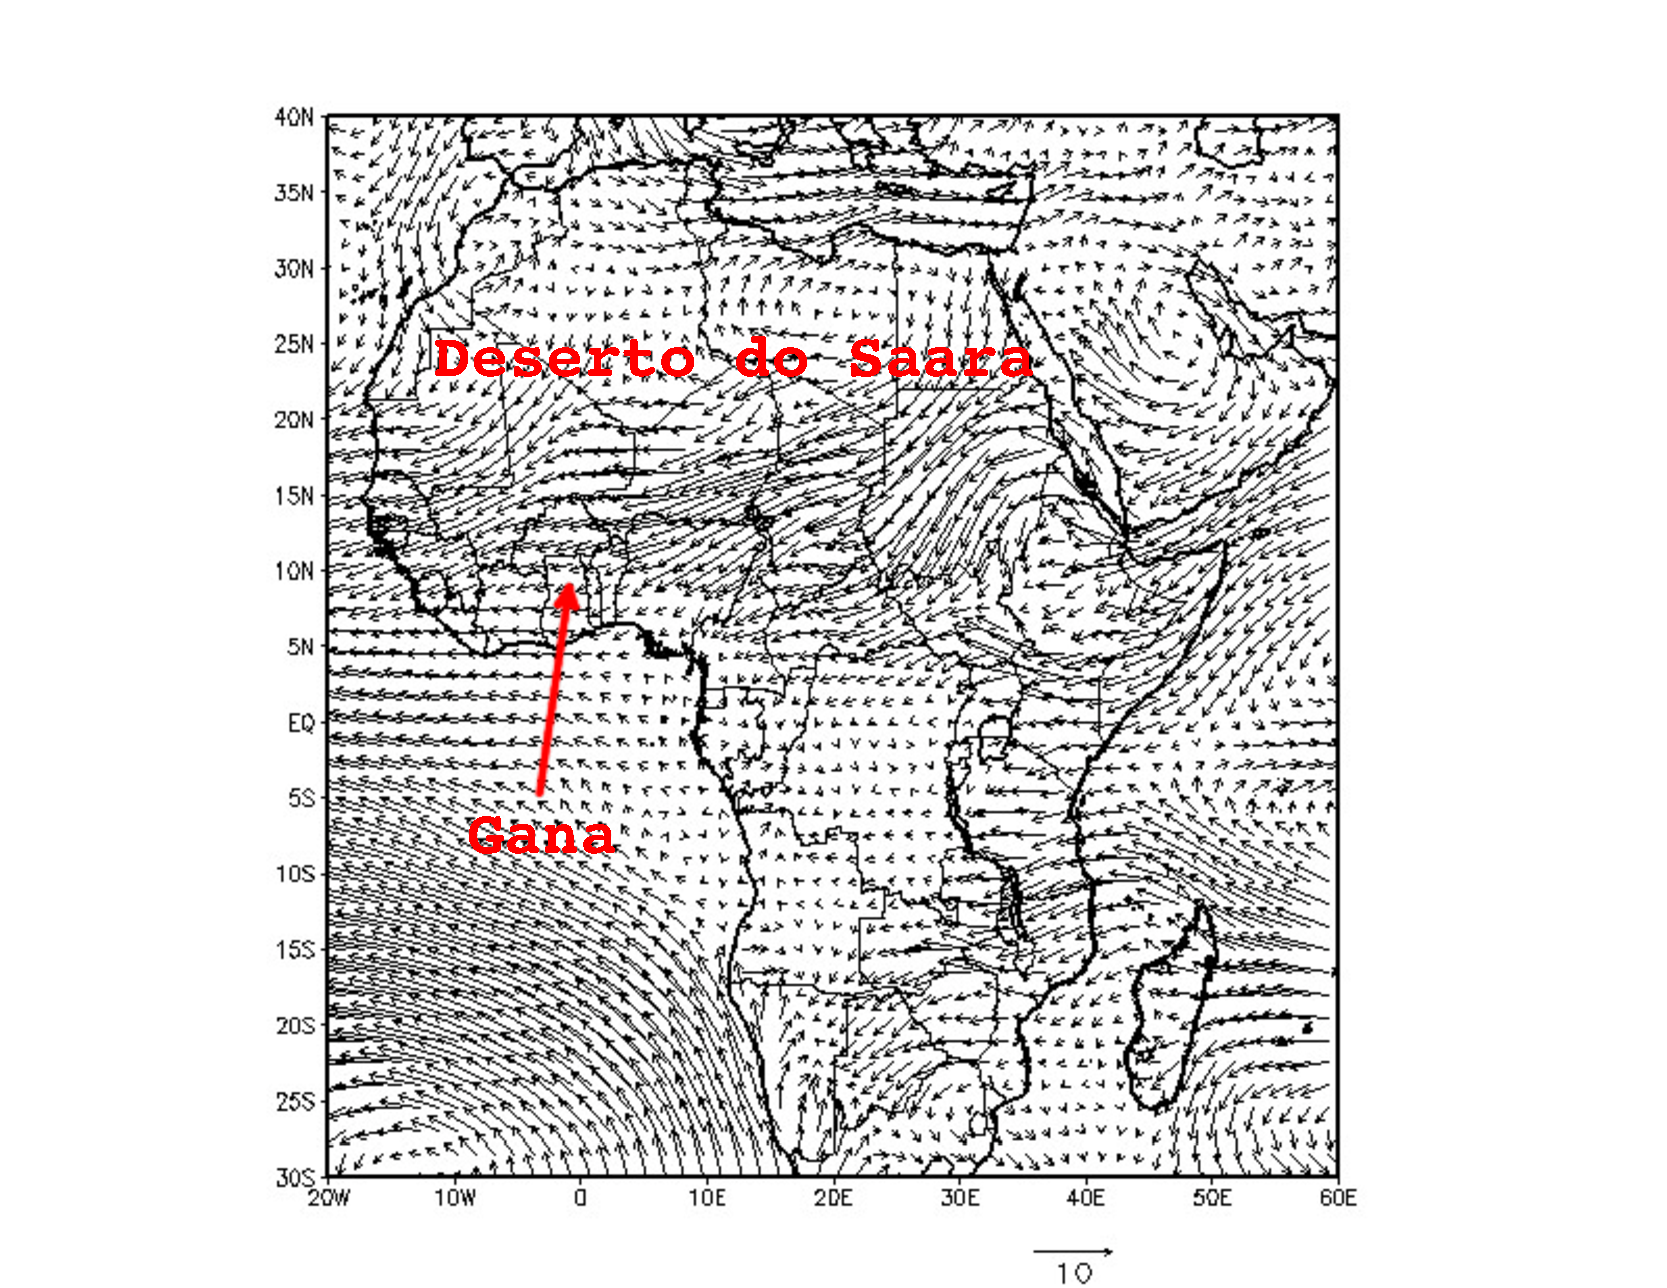
\includegraphics[width=\linewidth]{../inputs/grads/gimp/875hPa/DEZ_2007.pdf}
    \caption{Dezembro de 2007}
  \end{subfigure}%
%  \hspace{0.5cm}
  \begin{subfigure}[b]{0.5\linewidth}
    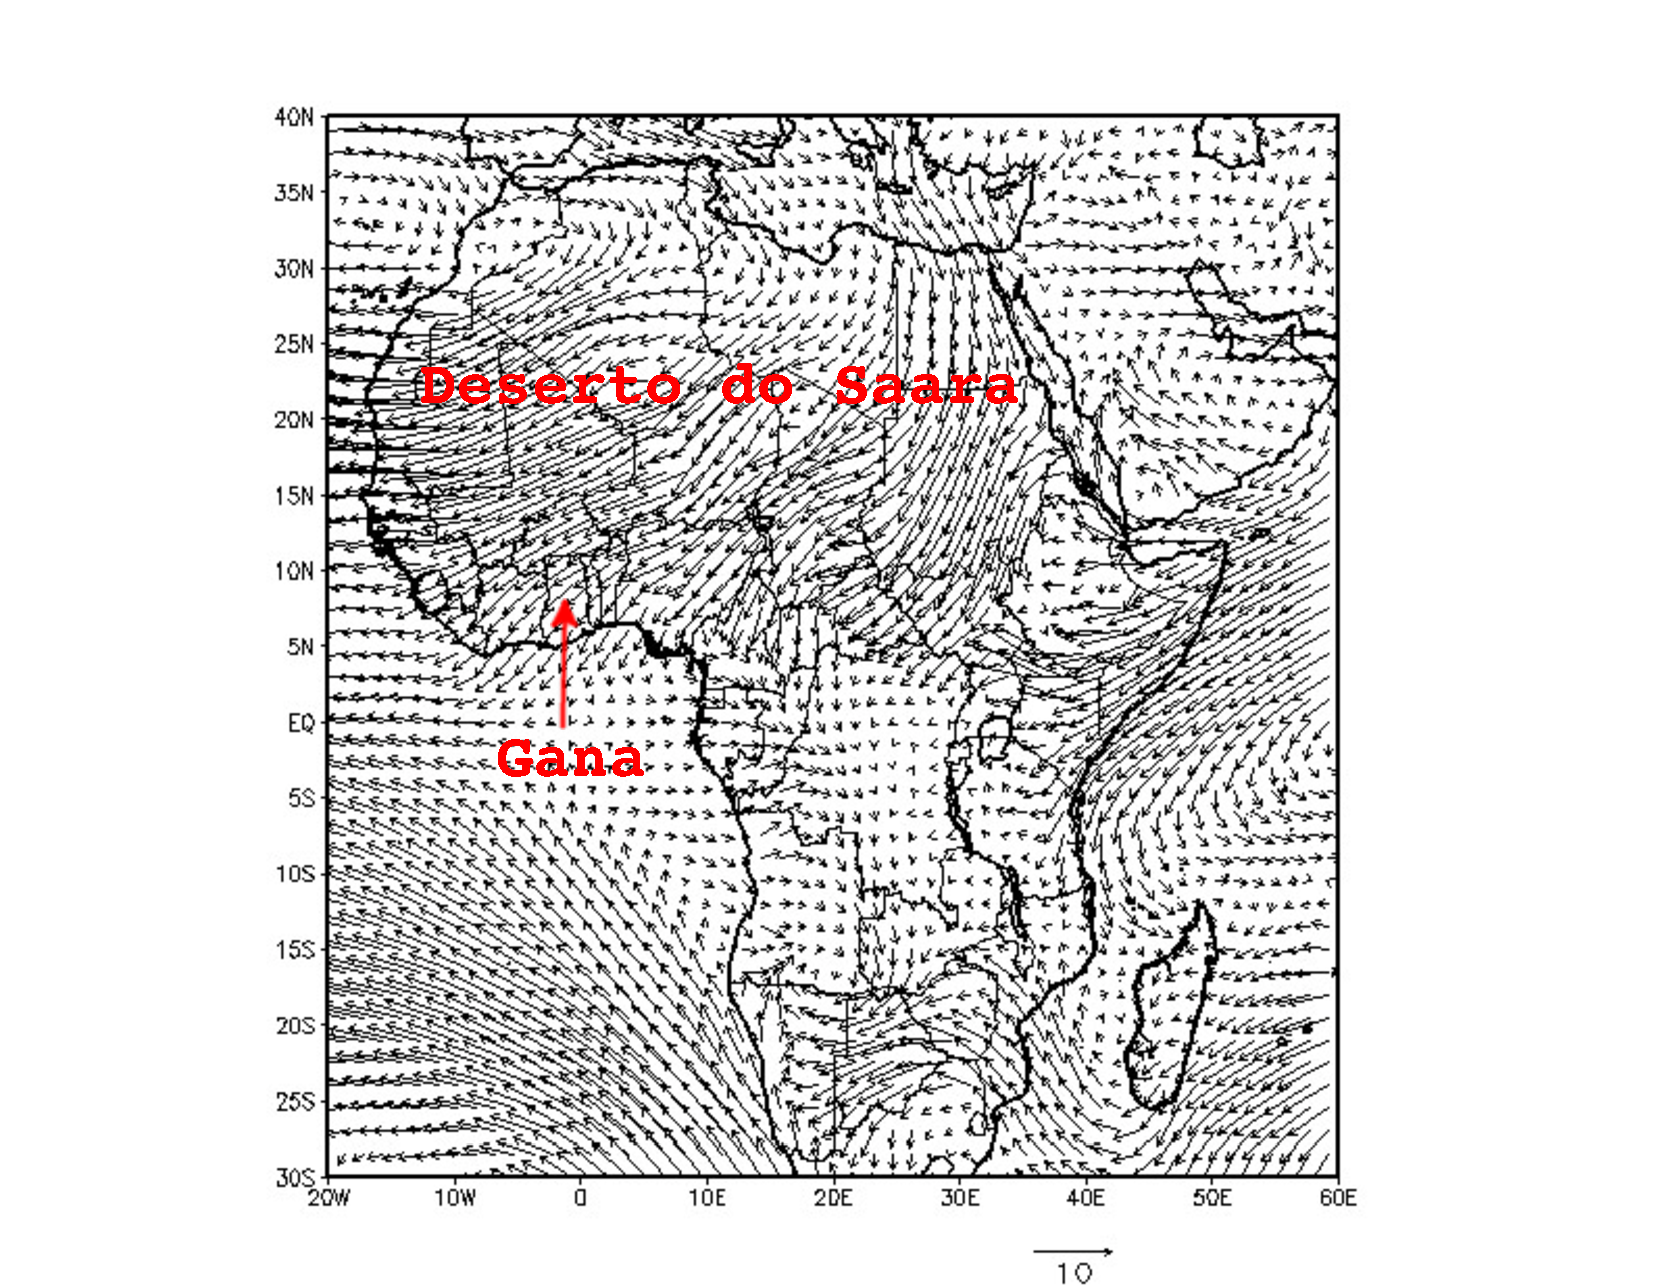
\includegraphics[width=\linewidth]{../inputs/grads/gimp/875hPa/JAN_2008.pdf}
    \caption{Janeiro de 2008}
  \end{subfigure}
  \caption{Intensidade e direção do vento predominante sobre o continente Africano
           em 875 hPa }
\end{figure}

\begin{figure}[H]
  \centering
  \begin{subfigure}[b]{0.5\linewidth}
    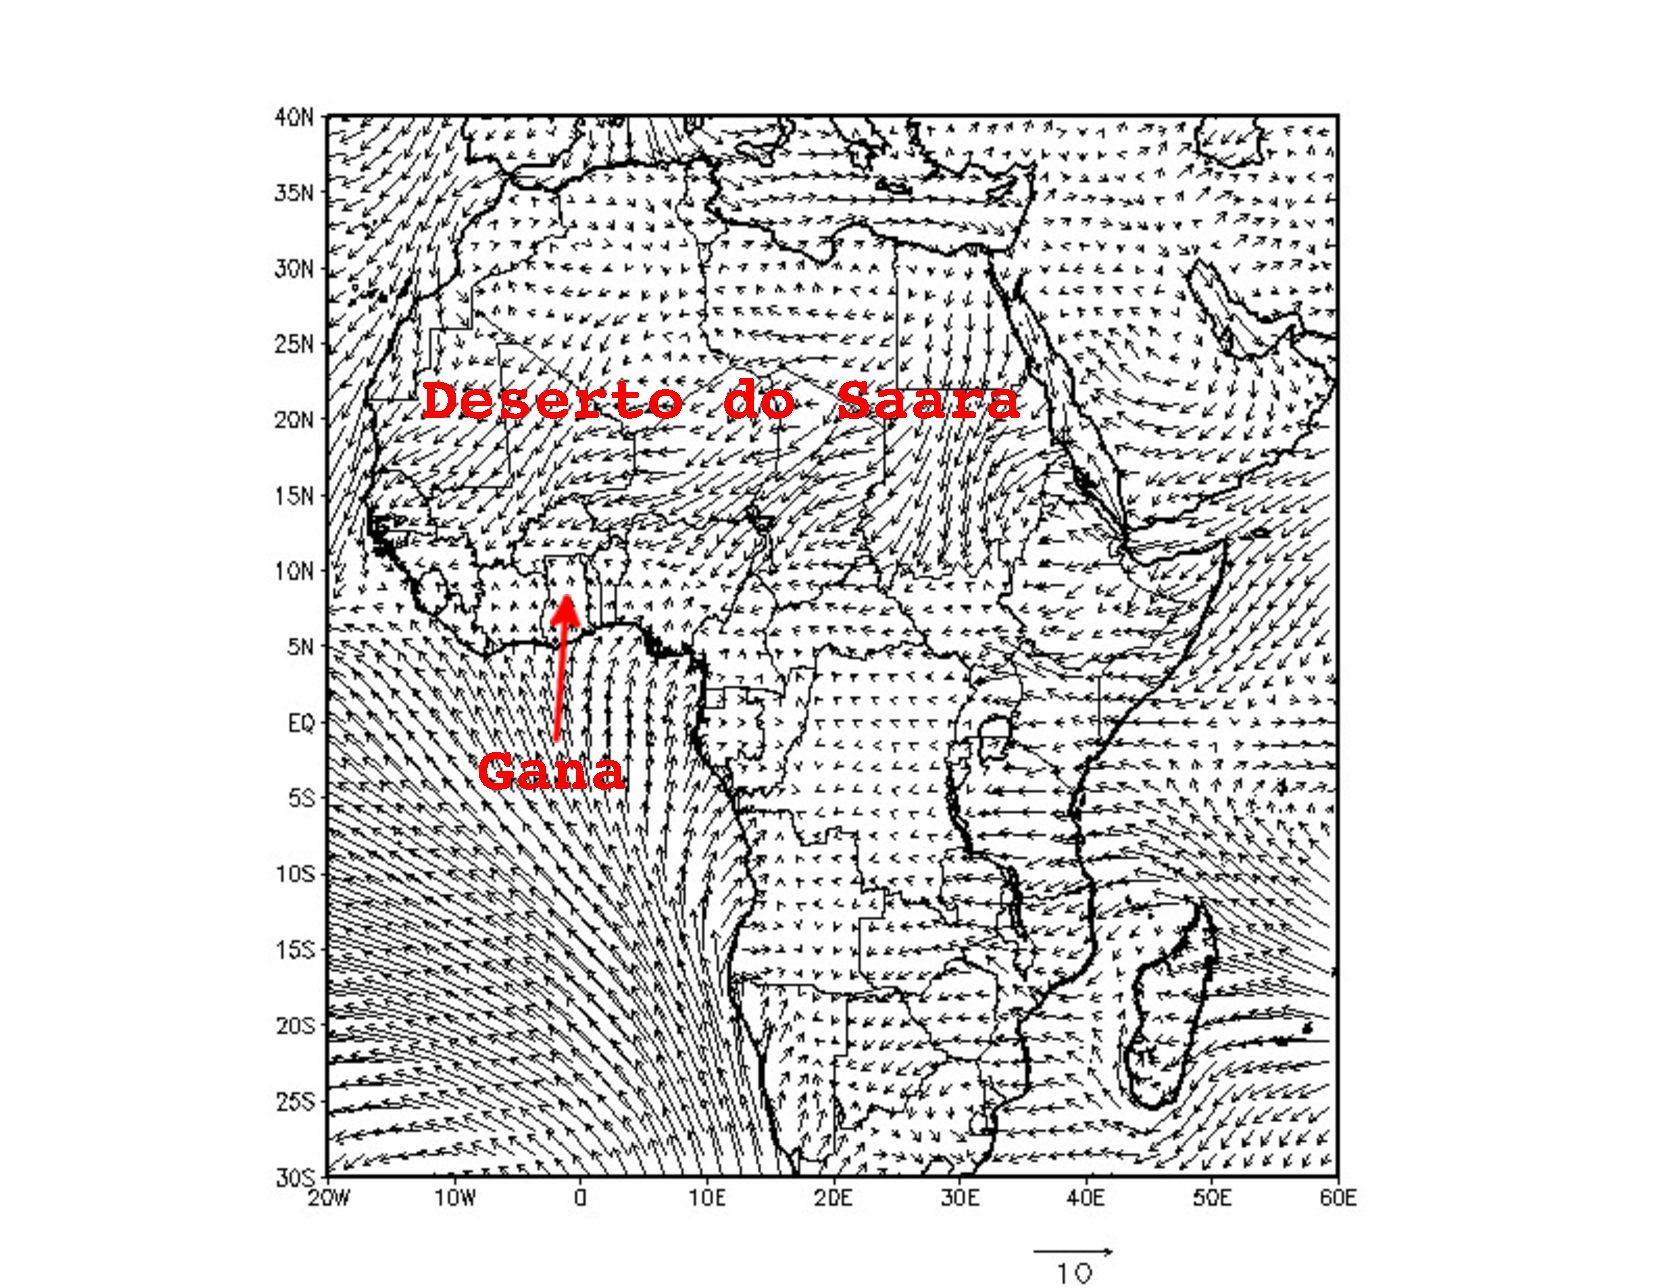
\includegraphics[width=\linewidth]{../inputs/grads/gimp/1000hPa/DEZ_2007.pdf}
    \caption{Dezembro de 2007}
  \end{subfigure}%
%  \hspace{0.5cm}
  \begin{subfigure}[b]{0.5\linewidth}
    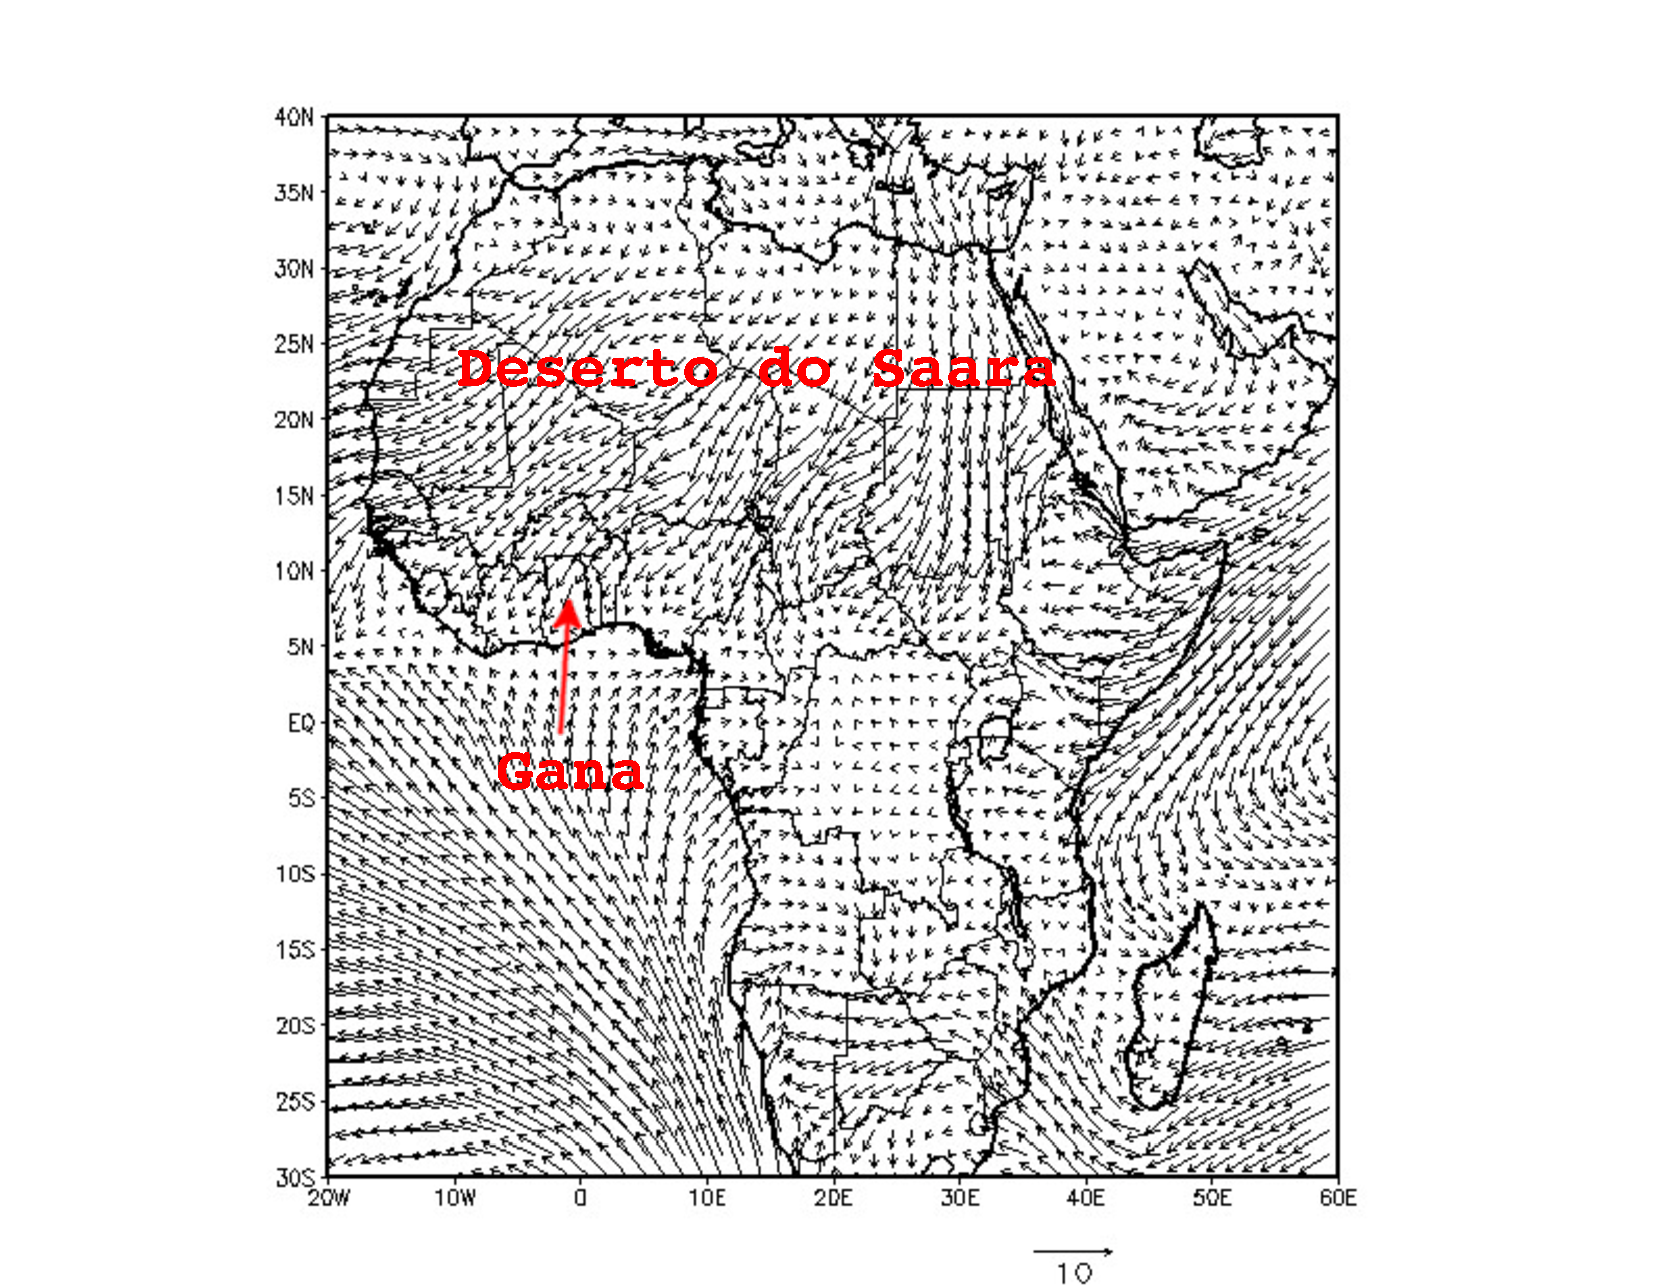
\includegraphics[width=\linewidth]{../inputs/grads/gimp/1000hPa/JAN_2008.pdf}
    \caption{Janeiro de 2008}
  \end{subfigure}
  \caption{Intensidade e direção do vento predominante sobre o continente Africano
           em 875 hPa}
\end{figure}

No Harmatão, a massa total de $MP_{10}$ mais que 500\%. Na área residencial, 
vai de 46,9 $\pm$ 1,4 $\mu g / m^3$ para 266,0 $\pm$ 34,0 $\mu g / m^3$
com a chegada do Harmatão (tabelas \ref{table:RIsH_descriptive} 
e \ref{table:RIeH_descriptive}) e na avenida de 67,1 $\pm$ 4,6 $\mu g / m^3$ 
para 272,0 $\pm$ 31,4 $\mu g / m^3$ (tabelas \ref{table:TIsH_descriptive} 
e \ref{table:TIeH_descriptive}). Esse é o motivo da legislação ambiental de Gana
ter limites mais permissivos durante esse período. 

Estudos como \citet{aboh2009}, \citet{ofosu2013}, \citet{ofosu2012} sugerem que
quando possível, isto é, com número de amostras suficientementes grande, excluir
dias do Harmatão nas análises estatísticas multivariadas, pois quando 
presentes, o Fator representante do Harmatão ofusca as fatores das fontes
locais.

O alto número de amostras coletadas em Nima, 879 no total, possibilitou a 
exclusão dos dias de ocorrência do Harmatão nas tabelas de concentrações 
sem comprometer as análises estatísticas multivariadas. 

Entretanto, o critério de exclusão não é simples, pois a poeira do Harmatão 
não é ininterrupta no período de ocorrência do mesmo. Classificando todos dias
de novembro até março como Harmantão, corre-se o risco de perde informações de 
fontes locais durante. Também não é possivel fazer essa classificação usando
a velocidade do vento, já que o fenômeno ocorre em altas altitudes. 

Uso-se o critério sugerido por \citet{aboh2009}, que considera os dias de 
ocorrência do Harmatão como os que tem concentrações de silício no $MP_{10}$ 
maiores que 10 $\mu g/m^3$, mas entre novembro e março. 54 amostras de $MP_{10}$
na área residencial e 59 na avenida foram classificadas como Harmantão. 



\newpage
\begin{table}[H]
  \centering
    \input{../outputs/descriptive_RIeH}
  \caption{Estatística descritiva das concentrações de $MP_{10}$ na área 
           residencial somente nos dias de ocorrência de vento Harmatão
          \label{table:RIeH_descriptive}}
\end{table}

\begin{table}[H]
  \centering
    \input{../outputs/descriptive_TIeH}
  \caption{Estatística descritiva das concentrações de $MP_{10}$ na área 
           residencial somente nos dias de ocorrência de vento Harmatão
           \label{table:TIeH_descriptive}}
\end{table}

\begin{landscape}
  \begin{figure}
    \centering
    \begin{minipage}[b]{0.45\linewidth}
      \includegraphics[width=\textwidth]{../outputs/RIeH_pmf_contribution_pizza4.pdf}
      \caption{Contribuição dos fatores na massa total para $MP_{10}$ na área
               residencial somente nos dias de ocorrência de vento Harmatão. seed = 123 n = 54.
               \label{fig:RIeH_contribution4}}
    \end{minipage}%\hfill
    \hspace{0.5cm}
    \begin{minipage}[b]{0.45\linewidth}
      \input{../outputs/RIeH_profiles_percent_species4.tex}
      \captionof{table}{Perfis do fatores para $MP_{10}$na área residencial,
                 somente nos de ocorrência de vento Harmatão. seed=123 e n= 54. 
                \label{table:RIeH_profiles4}}
    \end{minipage}
  \end{figure}
\end{landscape}

\begin{landscape}
  \begin{figure}
    \centering
    \begin{minipage}[b]{0.45\linewidth}
      \includegraphics[width=\textwidth]{../outputs/TIeH_pmf_contribution_pizza4.pdf}
      \caption{Contribuição dos fatores na massa total para $MP_{10}$ na avenida
               somente nos dias de ocorrência de vento Harmatão. seed = 123 n = 59.
               \label{fig:TIeH_contribution4}}
    \end{minipage}%\hfill
    \hspace{0.5cm}
    \begin{minipage}[b]{0.45\linewidth}
      \input{../outputs/TIeH_profiles_percent_species4.tex}
      \captionof{table}{Perfis do fatores na avenida $MP_{10}$ 
                 somente nos de ocorrência de vento Harmatão. seed=123 e n= 59. 
                \label{table:TIeH_profiles4}}
    \end{minipage}
  \end{figure}
\end{landscape}

%%%%
\subsection{Material Particulado Fino ($MP_{2,5}$)}

Resultados da Análise de Fatores e PMF para as tabelas de concentrações 
completas (com Harmatão) podem ser consultadas no apêndice II.

Os \textit{loadings} encontrados para Análise de Fatores de $MP_{2,5}$
na área residencial estão na tabela \ref{table:AF_RFsH5}, onde 83,58 \% 
da variância total dos dados foi explicada com 5 fatores retidos 
(o ideal é que se explique ao menos 80 \%) para uma base de dados de 123 amotras. 
O mesmo resultado, mas incluindo os dias de Harmatão, elevando para 197 amostras, 
disponível no apêndice II, tabela \ref{table:AF_RFcH5}, 90,8 \% da variância
foi explicada, mas há praticamente um fator predominante 
englobando a maioria dos elementos e explicando sozinho mais que 57,9 \% da 
variância total.

Na tabela \ref{table:AF_RFsH5}, apesar do primeiro fator continuar prepoderante,
ao menos os elementos estão melhor distribuídos entre os demais fatores.  

A comunalidade, variável que indica o quão o ajuste explicou a variabilidade por 
espécie, foi maior que $0,7$ para a maioria dos elementos,
com exceção do bromo (Br) e zinco (Zn) que tiveram comunalidade de $0,59$ e 
$0,44$, respectivamente.

No fator predominante, isto é, que explica sozinho a maior parte da variância 
43,78\%, tem altos \textit{loadings} para os metais (Al, Si, Ti, V, Fe, Mn, Ca, 
Mg) e massa. São oriundos de re-suspensão de poeira do solo e com exceção do 
Vanádio, são comumente encontrados em diversos tipos de solos, 
como os disponíveis no banco de dados SPECIATE da EPA-US \citep{simon2010}.
Ainda no primeiro fator, aparece secundariamente fósforo (P) e potássio (K), 
indicando possível sobreposição de fontes ou solo contaminado. 
Fósforo (P) e potássio (K), segundo SPECIATE, podem ser indicadores de 
fertilizantes. Gana não produz nenhum tipo de fertilizantes, mas importa para 
uso em fazenda locais \citep{fianko2011}. 
Vanádio, normalmente associado a queima de óleos pesados como o diesel, ao 
aparecer na fonte solo, indica sobreposição de fontes com temporalidade próximas.
\citet{aboh2009} também encontrou vanádio no fator de poeira solo em Acra, 
indicação que o solo é contamindado por vánadio.

As partículas que compõem poeira de solo estão em sua maioria na fração
grossa do Material Particulado ($MP_{2,5-10}$), pois são geradas por processo 
mecânico. Assim, é notável que mesmo no $MP_{2,5}$ é o principal fator, 
provavelmente explicável pelo grande número de ruas não pavimentadas em Acra. 

O segundo fator predominante explica 12,36 \% da variância total. 
Agrupa basicamente fósforo (P), potássio (K) e enxofre (S) e está relacionado
vegetação local, manipulação da terra e uso fertizantes. 
\citet{reid2005} aponta que o aparecimento de K,P,S e BC indicam queima de
biomassa, entretanto, o \textit{loading} do BC neste fator foi zero, o que nos
impede de supor que este fator esteja relacionado a queima de biomassa. 

O terceiro fator retido representa fonte veicular e explica 11,24\% da variância
total. É composto por Black Carbon (BC), chumbo (P), zinco (Zn), potássio (K) e 
massa. \citet{aboh2009} encontrou o mesmo fator em Kwabenya, 12km noroeste de 
Nima. BC e Zn estão associados a veículos, devido a combustão 
incompleta e desgaste das pastilhas de freio e dos pneus dos automóveis, 
respectivamente. O chumbo (Pb) foi banido da gasolina em Gana em 2003 devido 
a acordo internacional \citep{epa2015}.  
Na tabela \ref{table:RFcH_descriptive} a concentração média de $Pb$ 
foi $18,6 \pm 0,8 n g /m^3$, próximo de valores típicos encontrados em São Paulo 
$16 \pm 13 n g /m^3$ \citep{andrade2012}.

O quarto fator explica 8,81\% da variância, com Sódio (Na), Cloro (Cl) e
secundariamente enxofre (S) representa indubitavelmente a fonte mar. 
Partículas de Sódio (Na) e Cloro (Cl) geradas no mar estão mais concentradas 
na moda grossa ($MP_{2,5-10}$), mas pela proximidade do ponto de amostragem 
com mar, obteu-se concentrações suficientes que permitiram a geração de um fator. 
Em pouco tempo de residência na atmosfera, o Cloro do sal marinho envelhecido 
é substituído por $SO_4^{2-}$ como resultado da reação com ácido sulfúrico e 
ácido nítrico \citep{mcinnes1994}, o que explica a projeção do enxofre neste
fator (\textit{loading} de $0,29$).

O quinto e último fator retido explicou 7,40 \% da variância e agrupou
Bromo e Chumbo e representa queima de lixo sólido e outros materiais a céu 
aberto. 

Acra comporta um dos maiores lixões de eletrônicos (\textit{e-waste}) 
do mundo, recebendo grande parte dos equipamentos descartados como lixo na 
Europa e que são derretidos para obtenção do cobre (Cu) em Agbogbloshie, 
4 kilometros sudoeste de Nima.  

O zinco (Zn) é o principal composto de baterias de eletrônicos.Altas 
concentrações de Al, Co, Cu, Zn, Cd, In, Sb, Ba, e Pb foram encontradas
no solo do \textit{e-waste} de Agbogbloshie por \citet{asante2012},
que também observou altos nível de Fe, Sb, and Pb nas urinas de trabalhadores 
do de Agbogbloshie quando comparada a um pessoa de referência
(que não tenha tido contato com \textit{e-waste}).

Como pode ser observado na rosa dos ventos para o ano de 2007 
da figura \ref{fg:rosa2007} o vento predominante em Nima é de sudoeste, 
e portanto pode carregar material de Agbogbloshie para Nima. 
Assim, é possível que no fator 5, além da queima de lixo sólido local, 
também esteja representada pequena porção de contaminação do 
\textit{e-waste} de Agbogbloshie.

\begin{figure}[H]
  \centering
  \includegraphics[width=0.5\textwidth]{../outputs/windRose2007.pdf}
  \caption{Rosa do ventos para dados horários de 2007 do 
           Kotoka International Airport em Acra 
           \label{fg:rosa2007}}
\end{figure}%

%TODO: avaliar se usaremos o factor score para alguma coisa. 
%\newpage
%\begin{figure}[H]
%  \centering
%  \includegraphics[width=\textwidth]{../outputs/scores_RFsH5.pdf}
%  \caption{RGsH factor scores}
%\end{figure}

Na avenida, os resultados da Análise de Fatores de $MP_{2,5}$ estão na 
tabela \ref{table:AF_TFsH5}. Os fatores principais extraídos 
foram essencialmente os mesmos que na área residencial, apenas com mudanças nas
distribuições dos \textit{loadings} de alguns elementos, mas que não alteram 
as indicações de fontes já discutidas. Há um leve aumento do \textit{loading} 
do BC de 0,81 para 0,94 no fator de veículos, possivelmente relacionado a
maior movimentação de veículos na avenida.

\newpage
\begin{table}[H]
  \centering
  \input{../outputs/beautifulFAdisplay_RFsH5.tex}
  \caption{Análise de Fatores na área residencial para $MP_{2,5}$
           excluindo dias de ocorrência de vento Harmatão. n = 123.
          \label{table:AF_RFsH5}}
\end{table}

\begin{table}[H]
  \centering
  \input{../outputs/beautifulFAdisplay_TFsH5.tex}
  \caption{Análise de Fatores na avenida para $MP_{2,5}$
           excluindo dias de ocorrência de vento Harmatão. n = 122.
          \label{table:AF_TFsH5}}
\end{table}
\newpage

Para melhorar o apuramento de fontes de $MP_{2,5}$ apresenta-se também os
resultados das análises de PMF. Diversas parametrizações foram testadas no PMF 
e as soluções estáveis com fatores de significados físicos foram retidas. 
Foi adicionado 8\% da concentração na incerteza devido a amostragem paralela. 

A tabela \ref{table:RFsH_profiles5} apresenta o perfil dos fatores para a área
residencial de $MP_{2,5}$ e o gráfico da figura \ref{fig:RFsH_contribution5}
as respectivas contribuições do fatores na massa total. 

Assim como na Análise de Fatores, quando inclusos dias do Harmatão, 
o fator com elementos de poeira de solo se destaca de todos outros, 
pois sozinho contribuiu para 55,05\% da massa 
e carrega em seu perfil quase todos elementos, como pode ser observado 
no apendice I tabela \ref{table:RFcH_profiles5} e gráfico 
\ref{fig:RFcH_contribution5}.

Removendo-se o Harmatão o Fator 1 de perfil composto Black Carbon (BC), 
chumbo (Pb), zinco (Zn), potássio (K), $MP_{2,5}$, vanádio (V) e manganês (Mn).
Assim como na Análise de Fatores, representa fonte veicular, porém é que 
contribui mais para massa total 39,98 $\pm$1,93. É o fator de maior peso, 
o que é mais coerente do que se espera em $MP_{2,5}$, que o fator mais 
significativo seja de fontes de processos de combustão, que geram partículas
finas, e não solo, como encotrado na Análise de Fatores.

O fator 2, com 73\% da massa de bromo, 15,1\% de Pb e 15,1\% Zn representa 
queima de lixo sólido e outros materiais a céu aberto, não tendo contribuição
muito expressiva na massa total 4,65 $\pm$ 0,43 \%.

O fator 3 é o segundo que mais contribui para massa (22,18 $\pm$ 2,84 \%) 
e agrega os elementos identificados como poeira de solo Al, Si, Ti, V, Fe, Mn, 
Ca, Mg. Também aparece secundariamente fósforo (P), possível identificador de
fertilizantes. Enquanto que na Análise de Fatores o vanádio aparecia
quase que exclusivamente no fator poeira de solo no PMF sua massa está dividida
entre veículos (31,0\%) e solo (34,4\%), o que mostra que a distribuição
feita pelo PMF no caso do vanádio faz mais sentido com a realidade, já que
é normal encontrar vanánio em veículos movido a óleo pesado.

Contribuindo com 11,64 $\pm$ 0,89 \% da massa, o fator 4, composto por Na, Cl e
16,7 \% da massa do enxofre (S) corresponde a fonte marinha. 

O fator 5, mas o terceiro em contribuição na massa 21,55 $\pm$ 1,66 \%, depois
de veículo e poeira de solo, além do fósforo (P), potássio (K) e enxofre (S) 
encontrados no fator vegetação da Análise de Fatores, possui quase metade da 
massa do sódio 40,4 \%.

Os resultados para $MP_{2,5}$ do PMF para a avenida estão na tabela 
\ref{table:TFsH_profiles5} e no gráfico da figura \ref{fig:TFsH_contribution5}.

O fator 1 na avenida, quase que exclusivamente com toda massa do Bromo 68,4\%,
representa queima de lixo sólido, explicando apenas 3,86$\pm$0,37 \% da massa 
total.  

O fator 2, de contribuição 13,64 $\pm$ 1,06 \% corresponde a fonte marinha. 

O fator 3 é composto por elementos associados a ressuspensão de poeira de 
solo e contribuiu 22,23 $\pm$ 2,14) \% para massa total, praticamente
a mesma contribuição da área residencial. 

O fator 4, associado anteriormente a vegetação, teve aumento da massa de BC, 
de 19,6 \% para 31,6\% e também na contribuição da massa total, 
de 21,55 $\pm$ 1,66 para 28,82 $\pm$ 1,86) \%. A avenida XX, possui comércios
de venda de alimentos prontos para consumo, como churrasco, restaurantes, 
salgados, etc, que são majoritariamento produzidos por queima de biomassa. 
Para \citet{reid2005} K,P,S e BC segerem queima de biomassa, neste caso, 
acreditamos que o fator 4 representação vegetação e queima de biomassa.   

O fator 5, fonte veícular, teve sua contribuição na massa total relativa 
dimunuída de 39,98 $\pm$ 1,93 para 31,45 $\pm$ 1,83 \%, mesmo a avenida contendo 
movimentação de veículos superior a área residêncial,
dimunuição esta provavelmente devido ao aparecimento da fonte queima de biomassa. 

\begin{landscape}
  \begin{figure}
    \centering
    \begin{minipage}[b]{0.45\linewidth}
      \includegraphics[width=\textwidth]{../outputs/RFsH_pmf_contribution_pizza5.pdf}
      \caption{Contribuição dos fatores na massa total para $MP_{2,5}$ na área
               residencial excluindo dias de ocorrência de vento Harmatão. seed = 123 n = 123.
               \label{fig:RFsH_contribution5}}
    \end{minipage}%\hfill
    \hspace{0.5cm}
    \begin{minipage}[b]{0.45\linewidth}
      \input{../outputs/RFsH_profiles_percent_species5.tex}
      \captionof{table}{Perfis do fatores na área residencial $MP_{2,5}$ 
                 excluindo dias de ocorrência de vento Harmatão. seed=123 e n= 123. 
                \label{table:RFsH_profiles5}}
    \end{minipage}
  \end{figure}
\end{landscape}

\begin{landscape}
  \begin{figure}
    \centering
    \begin{minipage}[b]{0.45\linewidth}
      \includegraphics[width=\textwidth]{../outputs/TFsH_pmf_contribution_pizza5.pdf}
      \caption{Contribuição dos fatores na massa total para $MP_{2,5}$ na avenida
               excluindo dias de ocorrência de vento Harmatão. seed = 123 n = 122.
               \label{fig:TFsH_contribution5}}
    \end{minipage}%\hfill
    \hspace{0.5cm}
    \begin{minipage}[b]{0.45\linewidth}
      \input{../outputs/TFsH_profiles_percent_species5.tex}
      \captionof{table}{Perfis do fatores avenida $MP_{2,5}$ 
                 excluindo dias de ocorrência de vento Harmatão. seed=123 e n= 122. 
                \label{table:TFsH_profiles5}}
    \end{minipage}
  \end{figure}
\end{landscape}
 
%%%%
\subsection{Material Particulado Grosso $MP_{2,5-10}$}

Nas publicações referentes a este estudos \citet{ARKU2008} e 
\citet{DIONISIO2010} não houve separação entre $MP_{2,5}$ e $MP_{2,5-10}$. 
Nas amostras de Nima, essa separação foi feita, possibilitando a identificação
de fontes na fração grossa do material partículado. Lembra-se que o experimento
em paralelo com coleta de filtros de quartzo e posterior intercalibração de BC
só foi realizado para $MP_{2,5}$ e portanto não há medidas de BC para 
$MP_{2,5-10}$.

Os \textit{loadings} encontrados para Análise de Fatores de $MP_{2,5-10}$
na área residencial estão na tabela \ref{table:AF_RGsH5}. Com 112 
amostras explicou-se 93,36 \% da variância total dos dados, mas o número 
fatores retidos foi 4 e não 5 como no caso do fino. A comunalidade foi maior 
que $0,7$ para todos elementos.

O fator 1 explica sozinho quase metade da variância 49,07\% e tem 
projetados elementos componentes de poeira do solo Al, Si, Ti, Fe, Mn, Ca, 
Mg, mais $MP_{2,5-10}$ e contaminação de vanádio. Como é comum em $MP_{2,5-10}$, 
o solo é a fonte predominante. Nota-se que a poeira de solo foi presente 
tanto em $MP_{2,5-10}$ quanto em $MP_{2,5}$.

O fator 2 explica 24,25 \% da variância total e é formado por K, Zn, Pb, S, e 
Br. \citet{aboh2009} identificou em Kwabenya um fator (explicando 17\% da 
variância) composto por Zn, BC e Pb e o relacionou a uma mistura de 
fonte de industria local e queima de biomassa. O fator 2 aqui também será 
classificado como industria local e queima de biomassa. 

O terceiro fator explica 13,55\% da variância com altos \textit{loadings} de 
Na, Cl e S, representam se dúvida a fonte mar. 

O quarto e último fator composto por P e Zn representa industria local. 

Os resultados para Análise de Fatores de $MP_{2,5-10}$ na avenida expostos
na tabela \ref{table:AF_RGsH5} não diferem quase em nada daqueles encontrados
na área residencial, com pequenas mudaças nas projeções dos \textit{loadings}, 
como o caso do fósforo que passou do fator industria para o fator solo. 

\newpage
\begin{table}[H]
  \centering
  \input{../outputs/beautifulFAdisplay_RGsH4.tex}
  \caption{Análise de Fatores na área residencial para $MP_{2,5-10}$
           excluindo dias de ocorrência de vento Harmatão. n = 112.
          \label{table:AF_RGsH5}}
\end{table}

\begin{table}[H]
  \centering
  \input{../outputs/beautifulFAdisplay_TGsH4.tex}
  \caption{Análise de Fatores na avenida para $MP_{2,5-10}$
           excluindo dias de ocorrência de vento Harmatão. n = 116.
          \label{table:AF_TGsH5}}
\end{table}
\newpage

Os resultados de PMF para $MP_{2,5-10}$ na área residencial com extração de 
quatro fatores estão na tabela \ref{table:RGsH_profiles4} e gráfico 
\ref{fig:RGsH_contribution4}. Rápida olhada nos elementos dos fatores 1 e 2 
percebe-se que o PMF fez a separação do solo em dois, o primeiro com elementos
da crosta terrestre e um segundo solo contaminado com Zn, Pb e P. O terceiro 
fator é exclusivamente mar e o último mistura de queima de biomassa 
com industria. 

Repetindo a análise PMF mas com extração de 5 fatores obtém-se a tabela 
\ref{table:RGsH_profiles5} e o gráfico \ref{fig:RGsH_contribution5}.
Com extração de 5 fatores foi possível separar a queima de biomassa (fator 5)
das demais fontes e queima de lixo sólido (fator 1) das demais fontes. 
Nota-se que o solo continua separado em dois (fator 3 e 4) e a fonte mar está 
no fator 2. 

Na avenida, com extração de 4 fatores (tabela \ref{table:TGsH_profiles4} 
e gráfico \ref{fig:TGsH_contribution4}) apenas um solo é encontrados
(fator 3). Assim como na área residencial, é possível discriminar melhor 
os fatores relacionados a queima de biomassa ou lixo sólido se extrairmos 5
fatores no PMF. 

A tabela \ref{table:TGsH_profiles5} e e gráfico \ref{fig:TGsH_contribution5} 
mostram os resultados para o caso de 5 fatores extraídos na avenida. 
No fator 1 o mar ficou
bem definido, no fator 2, Mg, Fe e V, representa industria local. 

O fator 3 também reprenta alguma industria local (Zn, Pb e P).

No fator 4 estão juntos queima de biomassa e queima de lixo sólido a céu aberto. 
Por fim, o fator 5 representam poeira de ressuspensão de solo.  

\begin{landscape}
  \begin{figure}
    \centering
    \begin{minipage}[b]{0.45\linewidth}
      \includegraphics[width=\textwidth]{../outputs/RGsH_pmf_contribution_pizza4.pdf}
      \caption{Contribuição dos fatores na massa total para $MP_{2,5-10}$ na área
               residencial excluindo dias de ocorrência de vento Harmatão. seed = 123 n = 123.
               \label{fig:RGsH_contribution4}}
    \end{minipage}%\hfill
    \hspace{0.5cm}
    \begin{minipage}[b]{0.45\linewidth}
      \input{../outputs/RGsH_profiles_percent_species4.tex}
      \captionof{table}{Perfis do fatores na área residencial $MP_{2,5-10}$ 
                 excluindo dias de ocorrência de vento Harmatão. seed=123 e n= 112. 
                \label{table:RGsH_profiles4}}
    \end{minipage}
  \end{figure}
\end{landscape}

\begin{landscape}
  \begin{figure}
    \centering
    \begin{minipage}[b]{0.45\linewidth}
      \includegraphics[width=\textwidth]{../outputs/RGsH_pmf_contribution_pizza5.pdf}
      \caption{Contribuição dos fatores na massa total para $MP_{2,5-10}$ na área
               residencial excluindo dias de ocorrência de vento Harmatão. seed = 123 n = 123.
               \label{fig:RGsH_contribution5}}
    \end{minipage}%\hfill
    \hspace{0.5cm}
    \begin{minipage}[b]{0.45\linewidth}
      \input{../outputs/RGsH_profiles_percent_species5.tex}
      \captionof{table}{Perfis do fatores na área residencial $MP_{2,5-10}$ 
                 excluindo dias de ocorrência de vento Harmatão. seed=123 e n= 112. 
                \label{table:RGsH_profiles5}}
    \end{minipage}
  \end{figure}
\end{landscape}

%%%%

\begin{landscape}
  \begin{figure}
    \centering
    \begin{minipage}[b]{0.45\linewidth}
      \includegraphics[width=\textwidth]{../outputs/TGsH_pmf_contribution_pizza4.pdf}
      \caption{Contribuição dos fatores na massa total para $MP_{2,5-10}$ na avenida
               excluindo dias de ocorrência de vento Harmatão. seed = 123 n = 116.
               \label{fig:TGsH_contribution4}}
    \end{minipage}%\hfill
    \hspace{0.5cm}
    \begin{minipage}[b]{0.45\linewidth}
      \input{../outputs/TGsH_profiles_percent_species4.tex}
      \captionof{table}{Perfis do fatores avenida $MP_{2,5-10}$ 
                 excluindo dias de ocorrência de vento Harmatão. seed=123 e n= 116. 
                \label{table:TGsH_profiles4}}
    \end{minipage}
  \end{figure}
\end{landscape}

\begin{landscape}
  \begin{figure}
    \centering
    \begin{minipage}[b]{0.45\linewidth}
      \includegraphics[width=\textwidth]{../outputs/TGsH_pmf_contribution_pizza5.pdf}
      \caption{Contribuição dos fatores na massa total para $MP_{2,5-10}$ na avenida
               excluindo dias de ocorrência de vento Harmatão. seed = 123 n = 116.
               \label{fig:TGsH_contribution5}}
    \end{minipage}%\hfill
    \hspace{0.5cm}
    \begin{minipage}[b]{0.45\linewidth}
      \input{../outputs/TGsH_profiles_percent_species5.tex}
      \captionof{table}{Perfis do fatores avenida $MP_{2,5-10}$ 
                 excluindo dias de ocorrência de vento Harmatão. seed=123 e n= 116. 
                \label{table:TGsH_profiles5}}
    \end{minipage}
  \end{figure}
\end{landscape}


